\chapter{Doelstelling, opdracht en op te leveren resultaten voor het bedrijf}
%Als de aanleiding helder is geformuleerd beantwoord je de vraag naar ‘het waarom’ (doelstelling) en ‘het wat’ (de beoogde resultaten) van het project.
    %- Formuleer eerst de probleem dat het bedrijf heeft met dit project: welk probleem moet door of voor het bedrijf worden opgelost? Bijvoorbeeld: het probleem is dat klanten via teveel verschillende kanalen contact opnemen met het bedrijf waardoor er geen goed beeld is of de klant al afdoende is geholpen.
    %- Aansluitend daarop formuleer je de doelstelling. Bijvoorbeeld: het bedrijf heeft wil alle contacten met de klant via de website te laten lopen. Let daarbij op: de doelstelling kan veel groter zijn dan jij met je resultaat oplost, dit is soms een veel te grote klus als afstudeer- of projectopdracht. Het is voldoende als jouw resultaat er een bijdrage aanlevert.
    %- Deze doelstelling mondt uit in jouw opdracht. Wat ga je precies voor het bedrijf doen, en wat ga je opleveren? Jij hebt misschien als opdracht: Ontwerp een goede user-interface voor de website. Of: ontwerp een perfecte database. Zo’n opdracht kan een essentiële bijdrage leveren aan het behalen van de doelstelling.
    %- Formuleer welke concrete resultaten het bedrijf van jou wil krijgen als je project is afgelopen? Wat is af als het af is? Geef daarbij duidelijk aan welke vereisten op het moment van schrijven al bekend zijn. Het gaat dan bijvoorbeeld om programmeertaal, omgeving/platform. Mocht er al een ontwerpdocument of een concept meegeleverd worden met de opdracht, dan is dat een bijlage. Het is niet de bedoeling dat je zelf al ontwerpdocumentatie maakt in deze fase.
Zoals behandeld in het voorgaande hoofdstuk, duurt het claimproces van een verzekering te lang. Allianz wilt gebruik maken van de recent opkomende blockchain technologie om de huidig bestaande bedrijfsprocessen te automatiseren (zie figuur \ref{fig:allianz-blockchain}). Deze opdracht dient als afstudeeropdracht, waar het uiteindelijke doel de response tijd van een claim te verminderen waardoor er een betere klanttevredenheid komt.\par

De hoofddoelstelling van dit afstudeerproject is daarom het realiseren van een proof of concept (POC), die het E-ABS claim proces naar de blockchain verplaatst en de betalingen automatiseert. Hoewel de meeste aandacht uitgaat naar de POC wordt er in het begin van het project onderzoek gedaan naar de blockchain technologie, de verschillende mogelijke oplossingen en hoe informatie in een gedecentraliseerde applicatie veilig opgeslagen kan worden. Daarnaast wordt er in het begin analyse uitgevoerd op de huidige bedrijfsprocessen die vervangen worden en daarbij de realisatie van de nieuwe processen in het POC.

\begin{figure}[h!]
    \begin{center}
        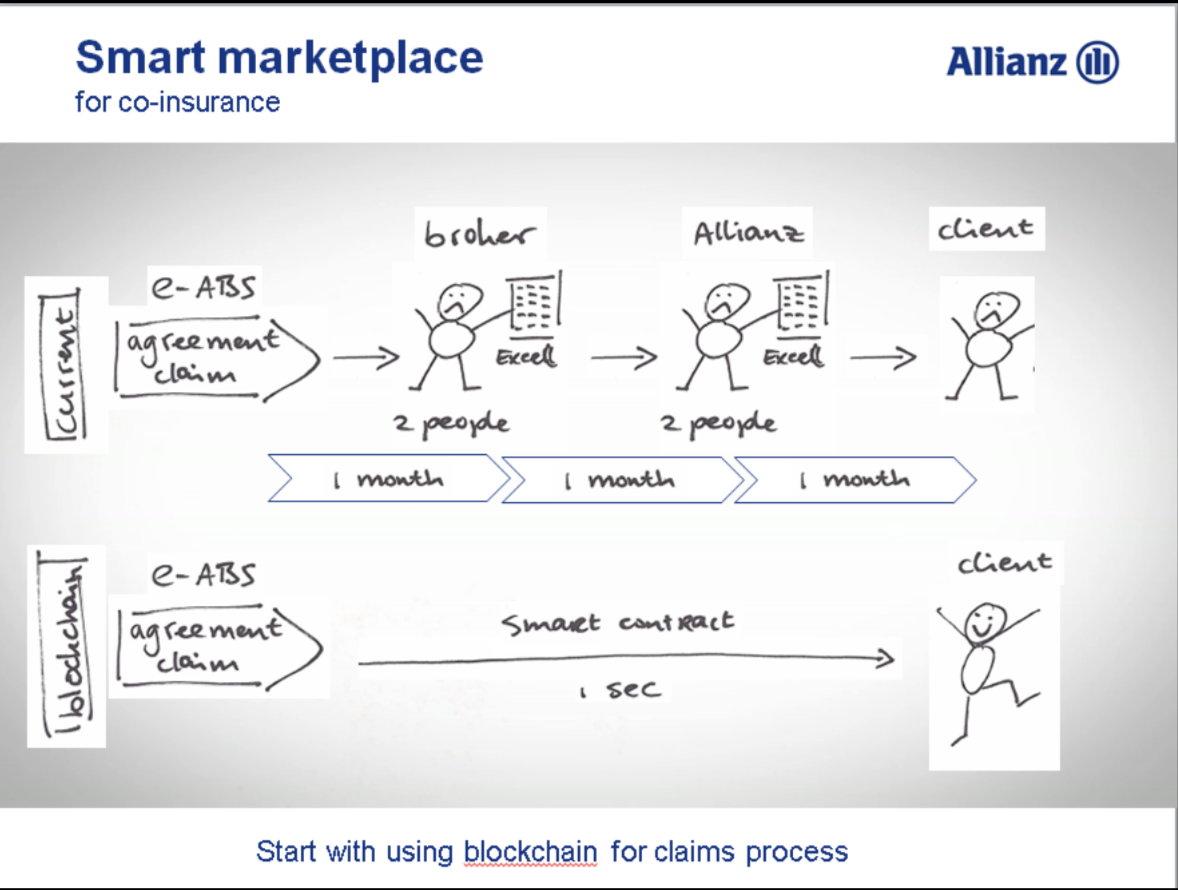
\includegraphics[scale=0.5]{images/allianz-blockchain}
        \caption{Usecase: co-insurance - Allianz}
        \label{fig:allianz-blockchain}
    \end{center}
\end{figure}

\section{Onderzoek}
Op het moment van schrijven het plan om onderzoek te doen naar het volgende hoofd- en deelvragen:
Hoofdvraag: ``\textit{Hoe automatiseer je het claim proces van Allianz door middel van de blockchain en smart contracts?}''\\
De volgende vragen komen aan bod:
\begin{itemize}
  \item Uit welke use cases en requirements bestaat het huidige proces van Allianz?
%  	\item Wat zijn de concerns van de stakeholders voor het claim proces?
  \item Wat is de blockchain?
  \item Welke kansen \& knelpunten bestaan bij het toepassen van de blockchain?
  \item Hoe automatiseer je het huidige proces met de blockchain?
\end{itemize}
De huidige hoofd- en deelvragen kan nog gedurende het onderzoek veranderen.